\section{An End-to-End Multi-Task and Fusion CNN for Inertial-Based Gait Recognition}

\begin{flushleft}
    \author{
    Rubén Delgrado-Esca$ \tilde{n} $o,
    Francisco M. Castro,
    Julián Ramos Cózar,
    Manuel J. Marín-Jiménez,
    and Nicolás Guil
    }
\end{flushleft}

\begin{center}
    \emph{IEEE DIGITAL OBJECT IDENTIFIER}
\end{center}

\subsection{INTRODUCTION}
An individual's gait appears as their own fingerprint. The study of this 
topic doesn't not only concern the area of medicine, but also that of security 
and identification. The gating study is based on a non-invasive system that 
collects patterns without the direct intervention of the subject. The data, 
which allow the recognition of the gait, are taken by inertial sensors present 
in a multitude of devices such as smartphones or smartwatches. A system 
is presented that uses a convolutional neural network (CNN) that uses the 
data collected by these inertial sensors to be able to predict the subject. The 
approach followed is the one in figure \ref{fig:preview}. Two extensions have been added 
to the network. The first deals with merging sensory data, while the second 
deals with improving the learning process and producing multiple outputs 
from a single input, thanks to a multi-task scheme. The tasks considered 
are: identification, gender recognition and age estimation. The dataset used 
is OU-ISIR gait database \cite{0857651721}, containing information such as inertial sensors 
such as accelerometers and gyroscopes. Gait recognition can be used in two contexts:
\begin{enumerate}
    \item {\bfseries{Identification}}: gait is used to obtain the identity of a known subject.
    \item {\bfseries{Authentication}}: gait is used to validate the identity of a known subject.
\end{enumerate}
\begin{figure}[htbp]
    \centering
    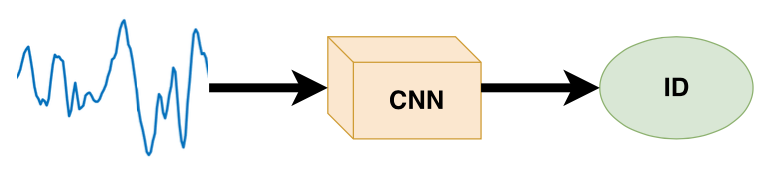
\includegraphics[width = 0.6 \linewidth]{images/paper5/usecase.png}
    \centering
    \caption{A preview of how the model works.}
    \label{fig:preview}
\end{figure}

\subsection{RELATED WORK}
Some methods have placed inertial sensors in different parts of the body 
such as legs \cite{0857651733}, hips \cite{0857651732}, ankles, or even in objects such as bags \cite{0857651735} and 
pockets \cite{0857651720}. Other methods \cite{0857651736} directly use all the inertial sensors present 
in the smartphone. With the advent of deep learning and CNNs, classifying 
an activity has turned out to be an easier job. The input provided to these 
networks is either the raw data of the inertial sensors, or the images that 
represented such data. The entire sequence of data is divided into segments, 
or windows, in order not to negatively affect the performance of the network. 
In the following work, a union of all the data produced by inertial sensors is 
carried out with the multi-task approach in order to provide a single model 
that uses different inputs to produce different outputs.

\subsection{PROPOSED APPROACH}
\subsubsection{Problem definition}
The proposed neural network is able to automatically extract the discriminat 
features from a gait sequence. There is no data pre-processing phase. The 
dataset used contains three labels for each fetature, indicating the age, years 
and gender of the subject, but in addition to this, any type of dataset with 
labels and sensory data would have been fine. In the following paper the 
following nomenclature will be used:
\begin{itemize}
    \item {\bfseries{\emph{S}}}: input temporal sequence of \emph{D} channel measurements taken by a sensor.
    \item {\bfseries{$ s_i $}}: sub-sequence of \emph{S} having length \emph{L}, given as input to CNN.
    \item $ y_i^t $: label of the sub-sequence $ s_i $ and taskt \emph{t}.
    \item $ g(s_i, \theta ) $: non-linear function applied to $ s_i $ with a set of parameters $ \theta $.
    \item {\bfseries{$ \hat{y_i} $}}: output of the network for a given $ s_i $ input.
\end{itemize}

\subsubsection{Initial CNN Architecture}
The length of the input is normalized before it can end up on CNN. Each 
sequence S is divided into U sub-sequences $ s_i $, where $ 1 \leq i \leq U $. However, 
a sequence is divided into windows having length L, with an overlap of 0\%, 
where each signal size defines a specific input channel. The number D of 
channels is useful for defining the 1 x N x D dimension of the filter of the 
first layer, where N indicates the dimension of the convolution. The proposed 
convolutional network is composed of 4 convolutional layers and a gradually 
increasing number of filters. After convolution there are elements such as 
ReLU, batch normalization (useful for faster learning) and max pooling. After 
the last convolutional layer, the average is chosen as a pooling operation. 
Then dropout and fully-connected layers are added with a number of outputs 
equal to the required classes. The last layer is composed of the Softmax 
normalization function which returns the probability distribution of each class. 
To train the model, only for the identification task, a cross-entropy is used 
as a loss function.
\begin{figure}[htbp]
    \centering
    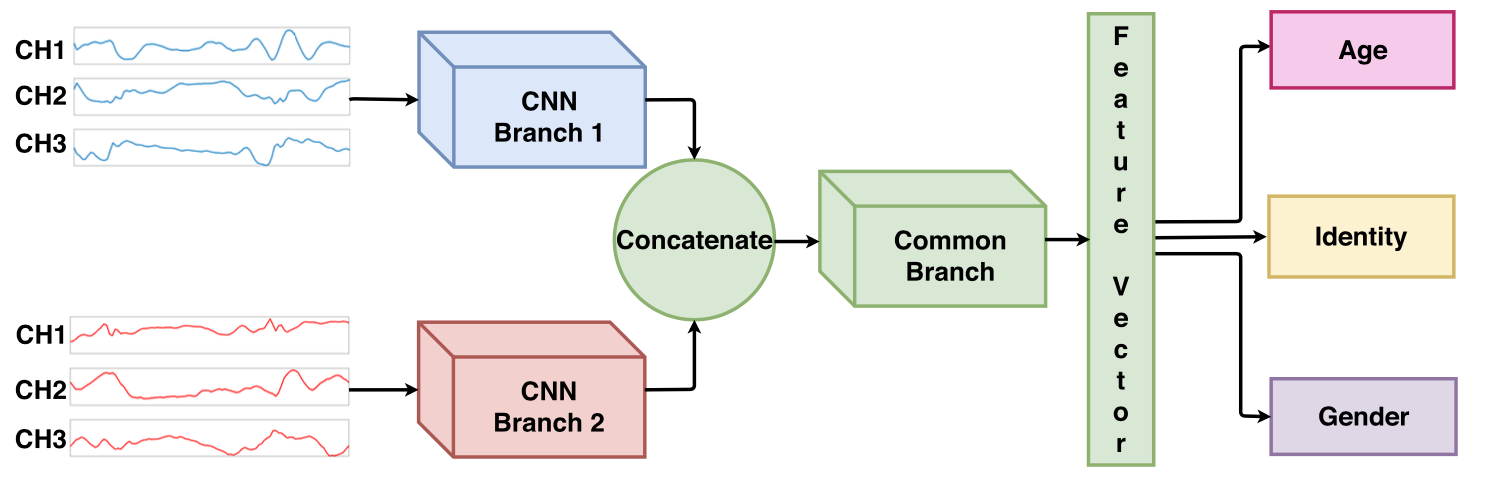
\includegraphics[width = 1 \linewidth]{images/paper5/architecture.png}
    \centering
    \caption{Pipeline for multi-task and multi-sensor learning in a gait-based system}
    \label{fig:pipeline}
\end{figure}

\subsubsection{Multi-task Approach}
The aim is to training a deep multi-task model (DTM). In order to do this, 
there must be a set of tuples $ I = (s_i, y_i^m, y_1^1, ..., y_i^T) $ where $ y_i^m $ is the label 
of the main task, $ y_i^t $, with $ t \in [1,T] $, is the label for each auxilary task. 
Each individual task has its own loss function \emph{L}. The loss function (\ref{loss-function}) is 
calculated on each sub-sequence \emph{s} and is formed by the product of each single 
loss function, of each task, with the weights ($ \lambda $)  associated at each task.
\begin{eqnarray}\label{loss-function}
    \emph{$ L_{DTM} (g(s,\theta), Y) $} & = & \lambda_{id}L_{id}(\hat{y}^{id}, y^{id}) \nonumber \\
                                        &   & + \lambda_{age}L_{age}(\hat{y}^{age}, y^{age}) \nonumber \\
                                        &   & + \lambda_{gender}L_{gender}(\hat{y}^{gender}, y^{gender}) 
\end{eqnarray}
Where $ Y = (y^{id}_i, y^{age}_i, y^{gender}_i) $ and $ L_{id}, L_{age}, L_{gender} $ are the loss functions of 
each tasks. As for the identity and gender tasks, their loss function is the 
cross-entropy and is calculated with the formula \ref{cross-entropy}.
\begin{equation}\label{cross-entropy}
    \emph{$ L_m(\hat{y}, c) $} = -\hat{y}_c+\log\sum^K_{k=1}e^{\hat{y}k} 
\end{equation}
Where $ \hat{y} $ is the ouput vector of the network, $ \hat{y}_c $ is the output for target class, 
$ \hat{y}_k $ is the \emph{k}-th component of the output vector, \emph{c} is the ground-truth class 
and \emph{K} is the total number of classes.

\subsubsection{Modality Fusion}
The merging of data that occurs at the input is useful for increasing the accuracy of the 
network and allows understanding the relationships between 
the different types of input data. Each data coming from a specific sensor 
will be inserted in an individual branch, composed of a specific number of 
convolutional layers that will calculate specific predictors for each sensor. 
In the end, the data will be concatenated in a common branch which has the 
task of extracting the combined features from all the sensors. Based on the accuracy metric, the 
layer that will return the best result will be selected.

\subsubsection{Identity Authentication}\label{IA}
An authentication process begins by submitting a sample of input to CNN. 
Within this, there may be a layer that will produce a vector of features. 
To find out which layer it is, a cross-validation process is performed. Once 
extracted, the features are normalized with the L2 standard. Subsequently 
a vector is calculated containing the Euclidean distances between the values 
given in input and those present in the training set. In order to calculate the 
\emph{Area Under Curve} (AUC) or the \emph{Equal-Error-Rate} (EER), these distances 
are transformed into probabilities.

\subsection{EXPERIMENTS AND RESULTS}
\subsubsection{Dataset}
The OU-ISIR dataset is composed in two parts. Part A contains data on 744 
individuals, each having two sub-sequence (s) recording at a rate of 100Hz 
via an IMU sensor located at the waist of each. The first sequence is used for 
training, the second for testing. The labels associated with each individual 
are: identity, gender and age (split in ranges). Part B, on the other hand, 
is composed of 495 individuals with 3 IMU sensors located on the body. For 
each individual and sensor, there are two sequences of walking levels, an up-slope 
walk sequence and the other down-slope walk. The data that will be 
merged are those coming from sensors such as accelerometer and gyroscope.

\subsubsection{Input data}
A data augumentation process is carried out to increase the amount of data 
available for training. In this way, instead of giving a single sequence S 
as input, three will be given, more precisely:
\begin{itemize}
    \item A Gaussian noise is added to the input signal;
    \item The sequence S is resized with a random value between 0.7 and 1.1;
    \item A sequence of 10 numbers is first interpolated to S and then the resulting sequence is sampled.
\end{itemize}
Each sequence (S) is divided into 100 sub-sequences ($ s_i $) (100Hz = 1 per 
second), a number enough to contain a walk, with overlap equal to 75\%.

\subsubsection{Implementation details}
First 100 epochs are performed in order to train the model, with the training 
set divided into training and validation. At the end of the training, in order to 
be able to fine-tune the parameters, a further 50 epochs are performed with 
the training set only. The optimization is carried out with the stochastic 
gradient descent (SGD) standard with a mini-batch of 128 samples, weigth 
decay of 0.0005 and a moment of 0.9. The total accuracy is obtained by 
combining the accuracies derived from the output of each sub-sequence ($ s_i $) 
of the input S. To obtain this, simply multiply each probability obtained 
from each of the sub-sequences with the following equation:
\begin{equation}
    P(S=c) = \prod_{i=1}^UP_i(s_i=c)
\end{equation}
Where U is the number of subsequences $ s_i $, P(s=c) is the probability of assign the identity \emph{c} to the person in sequence S and $ P_i(s_i=c) $ is the probability of assign the identity \emph{c} to teh person in subsequence $ s_i $.

\subsubsection{Gait Recognition experiments}
Different types of experiments on recognition, and their respective performances, in terms of accuracy and F1-measure, are presented below.
\begin{enumerate}
    \item \emph{Sensor position}: the following experiment show that using 3 different 
    sensors, the model has greater accuracy and a high value of F1-measure, 
    when using data from the sensor positioned on the left side of the body.
    \begin{table}[h!]
        \centering
        \begin{adjustbox}{max width=\textwidth}
        \begin{tabular}{*{3}{|c}|}%%{|c|c|c|}
            \hline
            IMU Position & Acc & F1-score \\
            \hline
            center & 92.3 & 90.8\\
            left & \bfseries{95.2} & \bfseries{94.0}\\
            right & 91.5 & 90.0\\
            \hline
        \end{tabular}
        \end{adjustbox}
        \caption{Accuracy and F1-score of three different sensors.}
        \label{table accuracy and F1}
    \end{table}

    \item \emph{Single task with individuals sensors} (1 Task, 1 Sensor): being a multi-task 
    network, a CNN network is created for each sensor in combination 
    with each label. As there are three types of labels and two sensors, a 
    total of 6 CNN networks are trained. From the results obtained from 
    the experiment, it can be seen that both sensors affect the model in an 
    almost similar way, in terms of accuracy and F1-Measure. These values 
    indicate that both sensors can be used in order to achive the purpose 
    of identifying the walk.
    \begin{table}[h!]
        \centering
        \begin{adjustbox}{max width=\textwidth}
        \begin{tabular}{|c||ccc|c||ccc|c|}
            \hline
                & \multicolumn{4}{c||}{Acc} & \multicolumn{4}{c|}{F1-Score} \\
            \hline
                Architecture & Id & Age & Gender & Avg & Id & Age & Gender & Avg\\
            \hline
                SingleTask Accelerometer & 89.7 & 91.0 & 94.8 & 91.8 & 87.6 & 91.3 & 94.5 & 91.2\\
                SingleTask Gyroscope& 89.1 & 89.1 & 94.4 & 90.9 & 87.5 & 89.7 & 94.4 & 90.5\\
            \hline 
        \end{tabular}
        \end{adjustbox}
        \caption{Accuracy and F1-score (1 Task, 1 Sensor).}
        \label{table accuracy and F1 (1 Task - 1 Sensor)}
    \end{table}

    \item \emph{Multi-task with individual sensors} (+ Task, 1 Sensor): in this experiment 
    more tasks are assigned to each of the sensors (3 tasks for 1 
    sensor) implying the creation of two CNN networks. This experiment 
    is useful to see if there are any performance improvements with respect 
    to the single assignment (defined in the previous point). The loss function 
    is that described in equation \ref{loss-function}. Comparing the results obtained 
    in table \ref{table accuracy and F1 (1 Task - 1 Sensor)} with table \ref{table accuracy and F1 (more Task - 1 Sensor)}, it can be seen that the following experiment led 
    to a slight improvement in performance.
    \begin{table}[h!]
        \centering
        \begin{adjustbox}{max width=\textwidth}
        \begin{tabular}{|c||ccc|c||ccc|c|}
            \hline
                & \multicolumn{4}{c||}{Acc} & \multicolumn{4}{c|}{F1-Score} \\
            \hline
                Architecture & Id & Age & Gender & Avg & Id & Age & Gender & Avg\\
            \hline
                MultiTask Accelerometer & 90.9 & 93.3 & 95.9 & 93.4 & 89.1 & 93.3 & 95.9 & 92.8\\
                MultiTask Gyroscope & 90.1 & 90.1 & 94.8 & 91.7 & 88.3 & 90.5 & 94.9 & 91.2\\
            \hline 
        \end{tabular}
        \end{adjustbox}
        \caption{Accuracy and F1-score (+ Task, 1 Sensor).}
        \label{table accuracy and F1 (more Task - 1 Sensor)}
    \end{table}

    \item \emph{Selection of the fusion position}: The fusion can take place in any convolutional 
    layer, called the common branch, of the network. For each 
    layer, a number of filters are applied which increases as the 
    depth of the network increases. As can be seen from table \ref{table accuracy and F1 fusion}, the best performances 
    are obtained in the fusion obtained in the first convolutional layer of 
    the network. Subsequent convolutional layers score lower because the 
    amount of information used for training is low.
    \begin{table}[h!]
        \centering
        \begin{adjustbox}{max width=\textwidth}
        \begin{tabular}{*{3}{|c}|}%%{|c|c|c|}
            \hline
            Position & Acc & F1-score\\
            \hline
            Conv1 & \bfseries{94.2} & \bfseries{92.9}\\
            Conv2 & 94.0 & 92.7\\
            Conv3 & 93.4 & 92.0\\
            Conv4 & 89.0 & 86.7\\
            Conv5 & 89.0 & 86.7\\
            \hline
        \end{tabular}
        \end{adjustbox}
        \caption{Accuracy and F1-score of fusion level experiment.}
        \label{table accuracy and F1 fusion}
    \end{table}

    \item \emph{Single Task with Fusion} (1 Task, + Sensor): in this experiment 3 CNNs 
    are used, one for each task, each making up a branch. In this case, the 
    combination of data from different sensors will be useful to be able to 
    determine only 1 task and therefore only one class. The results obtained 
    are better than the previous points, except for the gender class where 
    the MultiTask approach achieves a better score.
    \begin{table}[h!]
        \centering
        \begin{adjustbox}{max width=\textwidth}
        \begin{tabular}{|c||ccc|c||ccc|c|}
            \hline
                & \multicolumn{4}{c||}{Acc} & \multicolumn{4}{c|}{F1-Score} \\
            \hline
                Architecture & Id & Age & Gender & Avg & Id & Age & Gender & Avg\\
            \hline
                SingleTask Fusion & 94.2 & 95.0 & 95.6 & 94.9 & 93.5 & 95.0 & 95.6 & 94.7\\
            \hline 
        \end{tabular}
        \end{adjustbox}
        \caption{Accuracy and F1-score (1 Task, + Sensor).}
        \label{table accuracy and F1 (1 Task, + Sensor)}
    \end{table}

    \item \emph{Multi-task with Fusion} (+ Task, + Sensor): the last experiment consists in applying the fusion in a multitasking context within the network. In this case it will be necessary to train a CNN for all three existing tasks. From the results shown in table \ref{table accuracy and F1 (+ Task, + Sensor)}, this architecture manages to achieve better performance than the others mentioned above, this is because the model has much more information (labels and inputs) to describe people. The strength of this architecture is that it manages to return a result for each task.
    \begin{table}[h!]
        \centering
        \begin{adjustbox}{max width=\textwidth}
        \begin{tabular}{|c||ccc|c||ccc|c|}
            \hline
                & \multicolumn{4}{c||}{Acc} & \multicolumn{4}{c|}{F1-Score} \\
            \hline
                Architecture & Id & Age & Gender & Avg & Id & Age & Gender & Avg\\
            \hline
                MultiTask Fusion & \bfseries{94.8} & \bfseries{96.1} & \bfseries{97.7} & \bfseries{96.2} & \bfseries{93.8} & \bfseries{96.3} & \bfseries{97.7} & \bfseries{95.9}\\
            \hline 
        \end{tabular}
        \end{adjustbox}
        \caption{Accuracy and F1-score (+ Task, + Sensor).}
        \label{table accuracy and F1 (+ Task, + Sensor)}
    \end{table}
\end{enumerate}

\subsubsection{Authentication Experiments}
In paragraph \ref{IA} we said that to see if two different samples belong to the 
same subject, an identity authentication process must be carried out. In 
other words, it is necessary to evaluate the goodness of a model by calculating 
the AUC and EER index. To do this, one had to first calculate the 
Euclidean distances between the sample vector present in the test set with 
the sample vectors present in the training set. Subsequently, it was necessary 
to transform these distances into probabilities that will be represented 
on a ROC curve. Once this is done, for each model previously described, 
the values for AUC (the higher the better) and EER (the lower the better), 
calculated on the ROC curve, are shown in table \ref{Authentication}. From the results shown 
in the table, the multitask model obtains worse performance than the singletask 
model, this is caused by the fact that in the multitask model the labels 
to be managed are many more than the single label (id) to be managed in 
the singletask model.
\begin{table}[h!]
    \centering
    \begin{adjustbox}{max width=\textwidth}
    \begin{tabular}{|c|cc|}
        \hline
        Architecture & EER & AUC\\
        \hline
        SingleTask Accelerometer & 1.47 & 99.91\\
        SingleTask Gyroscope & 2.50 & 99.80\\
        \hline
        MultiTask Accelerometer & 1.61 & 99.90\\
        MultiTask Gyroscope & 2.85 & 99.72\\
        \hline
        SingleTask Fusion & \bfseries{1.14} & \bfseries{99.93}\\
        \hline
        MultiTask Fusion & 1.34 & 99.92\\
        \hline
    \end{tabular}
    \end{adjustbox}
    \caption{Authentication accuracy.}
    \label{Authentication}
\end{table}

\subsubsection{State of art comparison}
Comparing the proposed system with those already existing in the state of 
art, both for gait recognition (Tab.\ref{Gait comparison}) and authentication (Tab.\ref{Authentication comparison}), the 
performances outperforms those of the competitors.
\begin{table}[h!]
    \centering
    \begin{adjustbox}{max width=\textwidth}
    \begin{tabular}{|c|ccc|c|}
        \hline
        CNN & Id & Age & Gender & Avg\\
        \hline
        AE-GDI-CC & 61.0 & - & - & -\\
        Muaaz et al. & 63.5 & - & - & -\\
        Ngo et al. & 70.2 & - & - & -\\
        Wei et al. & 83.8 & - & - & - \\
        \hline
        MultiTask Fusion & \bfseries{94.8} & \bfseries{96.1} & \bfseries{97.7} & \bfseries{96.2}\\
        \hline
    \end{tabular}
    \end{adjustbox}
    \caption{Gait recognition comparison with some methods.}
    \label{Gait comparison}
\end{table}

\begin{table}[h!]
    \centering
    \begin{adjustbox}{max width=\textwidth}
    \begin{tabular}{|c|c|}
        \hline
        Approach & EER\\
        \hline
        Gafurov et al. & 15.8 \\
        Derawi et al. & 14.3 \\
        Rong et al. & 14.3 \\
        Ngo et al. & 13.5 \\
        Imp GDI + i-vector & 7.1 \\
        NC GDI + i-vector & 5.6 \\
        \hline
        SingleTask Fusion & \bfseries{1.1}\\
        \hline
    \end{tabular}
    \end{adjustbox}
    \caption{Authentication comparison with some methods.}
    \label{Authentication comparison}
\end{table}

\subsubsection{Execution time during test}
MultiTask models are the most time-consuming, but it is also true that they 
produce three outputs simultaneously (Fig. \ref{fig:time}).
\begin{figure}[htbp]
    \centering
    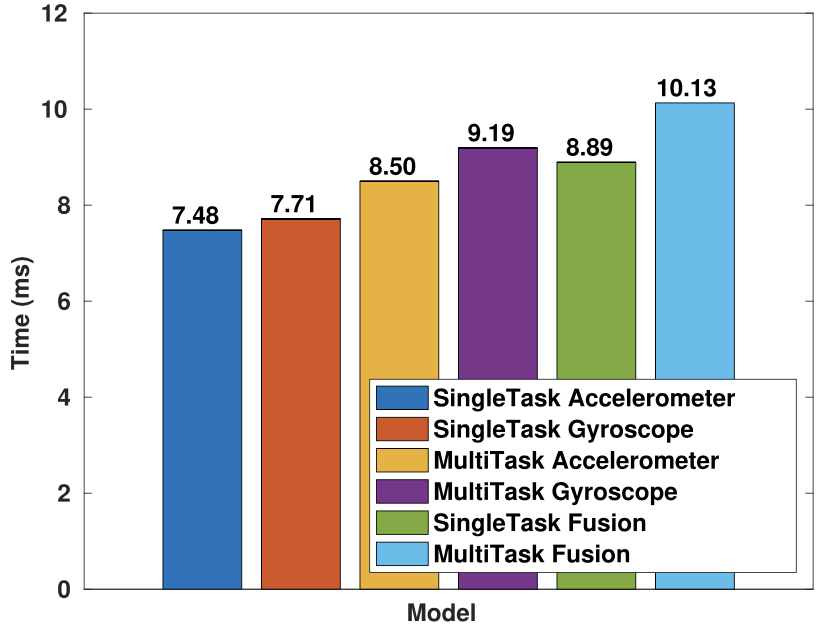
\includegraphics[width = 0.6 \linewidth]{images/paper5/time.png}
    \centering
    \caption{Execution time of the proposed models}
    \label{fig:time}
\end{figure}

\subsection{CONCLUSIONS}
As a final consideration, the model to be used, in the case of gait recognition, 
is the one that merges the input information and adopts a multitask 
approach. On the other hand, as regards the authentication problem, it has 
been seen that it is better to use a singletask model.